\chapter{Gauge invariance of heat transport coefficients} \label{ch:gauge-invariance}

It is often implicitly assumed that the well-definiteness of thermal transport coefficients would stem from the uniqueness of the decomposition of the system's total energy into localized, atomic, contributions. This assumption is manifestly incorrect, as any decomposition leading to the same value for the total energy as Eq.~\eqref{eq:atomic-energies} should be considered as legitimate. The difficulty of partitioning a system's energy into subsystems' contributions is illustrated in Fig.~\ref{fig:energy-partition}, which depicts a system made of two interacting subsystems. When defining the energy of each of the two subsystems, an arbitrary decision has to be made as to how the interaction energy is partitioned. In the case depicted in Fig.~\ref{fig:energy-partition}, for instance, the energy of each of the two subsystems can be defined as $\mathcal{E}(\rOmega_i) = E(\rOmega_i) + \frac{1}{2}(1\pm\lambda)W_{12}$, where $E(\rOmega_i)$ are the energies of the two isolated subsystems, $W_{12}$ their interaction energy, and $\lambda$ an arbitrary constant. In the thermodynamic limit, when all the subsystems' energies are much larger than the interaction between any pairs of them, the value of the $\lambda$ constant is irrelevant. When it comes to defining energy densities (\emph{i.e.} energies of infinitesimal portions of a system) or atomic energies, instead, the magnitude of the interaction between different subsystems is comparable to their energies, which become therefore intrinsically ill-defined.

\begin{figure}
\begin{minipage}{0.5\textwidth}
\centering 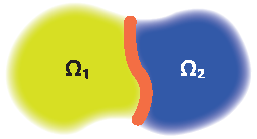
\includegraphics{chapters/chapter3/figures/blob.pdf}
\end{minipage}
\begin{minipage}{0.4\textwidth}
\begin{align*}
  E(\rOmega_{1}\cup\rOmega_2) &= E(\rOmega_1) + E(\rOmega_2) + W_{12} \qquad \\
  & \overset{?}{=}\mathcal{E}(\rOmega_1)+\mathcal{E}(\rOmega_2)
\end{align*}
\end{minipage}
\caption{
	The energy of an isolated system is the sum of the energies of its subsystems (as defined when they are isolated as well) plus the interaction among them, $W_{12}$, whose magnitude scales as the area of the interface, depicted in red. When defining the energies of individual subsystems, $\mathcal{E}$, $W_{12}$ has to be arbitrarily partitioned among them. \label{fig:energy-partition}}
\end{figure}

Let us consider a mono-atomic fluid interacting through pair potentials, $v(|\mathbf{R}_n-\mathbf{R}_m|)$, and define the atomic energies as \citep{Marcolongo2014,Ercole2016}:
\begin{equation}
  e_{\smallgamma,n}(\rGamma) =
  \frac{1}{2M_n}(\mathbf{P}_{n})^{2} + \frac{1}{2}\sum_{m\ne n}
  v(|\mathbf{R}_{n}-\mathbf{R}_{m}|)
  (1+\gamma_{nm}), \label{eq:Lambda-atomic-energies}
\end{equation}
where $\gamma_{nm}=-\gamma_{mn}$ is \emph{any} antisymmetric matrix.
As the inter-atomic potential appearing in Eq.~\eqref{eq:Lambda-atomic-energies} is symmetric with respect to the atomic indices, it is clear that the sum of all the atomic energies does not depend on $\gamma$, thus making any choice of $\gamma$ equally permissible. This trivial observation has deep consequences on the theory of thermal fluctuations and transport, because the value of the macroscopic energy flux, instead, depends explicitly on $\gamma$, thus making one fear that the resulting transport coefficients would depend on $\gamma$ as well. Using the same manipulations that lead from Eqs.~\eqref{eq:epsilon-classical} and \eqref{eq:atomic-energies} to Eq.~\eqref{eq:J-classical}, for any choice of the $\gamma$ matrix in Eq.~\eqref{eq:Lambda-atomic-energies}, a corresponding expression for the macroscopic energy flux can be found, reading \citep{Marcolongo2014,Ercole2016}:
\begin{equation}
  \mathbf{J}_{\smallgamma}^\smallE=\mathbf{J}^\smallE+
  \frac{1}{2 \rOmega}\sum_{n,m\ne n}\gamma_{nm} \Bigl ( v_{nm} \mathbf{V}_{n} + \bigl (\mathbf{V}_{n}\cdot \nabla_{\mathbf{R}_n} v_{nm} \bigr )  (\mathbf{R}_{n}-\mathbf{R}_{m}) \Bigr ), \label{eq:Lambda-classical-current}
\end{equation}
where $v_{nm}= v(|\mathbf{R}_{n} - \mathbf{R}_{m}|)$.

\begin{figure}
    \begin{center}
        \subfigure[\label{fig:argon-gauge-acf}]{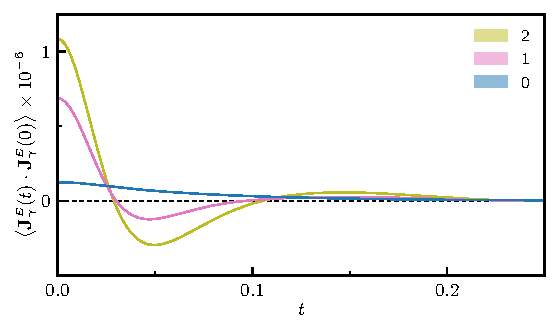
\includegraphics[width=10cm]{chapters/chapter3/figures/handbook_argon_egauge_acf.pdf}}
        \subfigure[\label{fig:argon-gauge-kappa}]{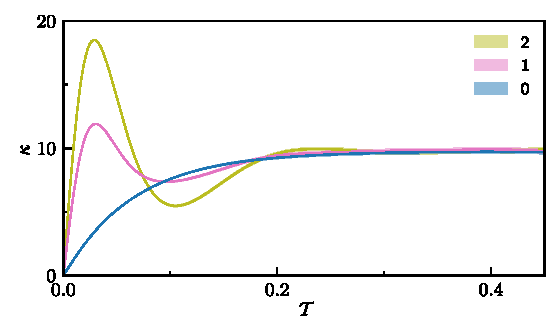
\includegraphics[width=10cm]{chapters/chapter3/figures/handbook_argon_egauge_kappa.pdf}}
    \end{center}
	\caption{(a) Time correlation functions of the modified macroscopic energy flux of a Lennard-Jones fluid, at the conditions described in the text, as defined in Eq.~\eqref{eq:Lambda-classical-current}, for different definitions of the $\gamma$ matrix. The ``0'' line refers to the standard definition ($\gamma = 0$), whereas the labels ``1'' and ``2'' correspond to two other (arbitrary) definitions of $\gamma$ as described in \cite{Ercole2016}.
    (b) Integral of the time correlation functions displayed in Fig.~\ref{fig:argon-gauge-acf}, multiplied by the prefactor appearing in the GK relation, Eq.~\eqref{eq:GK-complete}, as a function of the upper limit of integration. The barely visible shaded area surrounding each line is an indication of the error bars, as estimated by standard block analysis. Units are Lennard-Jones units ($M=\sigma=\varepsilon=1$). \label{fig:argon-gauge}}
\end{figure}

As a specific example, \cite{Ercole2016} ran MD simulations for a Lennard-Jones monoatomic fluid described by the inter-atomic potential $v(r)=\epsilon \left [ \left ( \frac{\sigma}{r}\right )^{12} - \left ( \frac{\sigma}{r}\right )^{6}\right ] $ at temperature $T=1.86 \frac{\epsilon}{k_B}$ and density $\rho=0.925 \sigma^{-3}$. In Fig.~\ref{fig:argon-gauge-acf} we display the resulting macroscopic energy-flux autocorrelation function corresponding to different choices of the $\gamma$ matrix in Eqs.~\eqref{eq:Lambda-atomic-energies} and \eqref{eq:Lambda-classical-current}. Fig.~\ref{fig:argon-gauge-acf} clearly shows that the $\langle \mathbf{J}^\smallE_{\gamma}(t) \cdot\mathbf{J}^\smallE_{\gamma}(0) \rangle$ correlation functions dramatically depend on the $\gamma$ matrices in Eqs.~\eqref{eq:Lambda-atomic-energies} and \eqref{eq:Lambda-classical-current}.  Notwithstanding, the integrals of all these time correlation functions tend to the same limit at large integration times, as shown in Fig.~\ref{fig:argon-gauge-kappa}.

In order to get insight into this remarkable invariance property, let us inspect the difference between the generalized flux in Eq.~\eqref{eq:Lambda-classical-current} and the standard expression of Eq.~\eqref{eq:J-classical}:
\begin{equation}
  \rDelta\mathbf{J}^\smallE_{\smallgamma} =\mathbf{J}^\smallE_{\smallgamma}-\mathbf{J}^\smallE  =\frac{\mathrm{d}}{\mathrm{dt}}\frac{1}{4 \rOmega} \sum_{n,m\ne n}  \gamma_{nm} \, v(|\mathbf{R}_{n}-\mathbf{R}_{m}|)  (\mathbf{R}_{n}-\mathbf{R}_{m}). \label{eq:DeltaJ}
\end{equation}
We see that the two different expressions for the macroscopic energy flux differ by a total time derivative of a bounded phase-space vector function. In the following, we show that this is a consequence of energy conservation and extensivity and a sufficient condition for the corresponding thermal conductivities to coincide.

The very possibility of defining an energy current density, from which the energy fluxes of Eq.~\eqref{eq:J-classical} and \eqref{eq:Lambda-classical-current} ultimately depend, stems from energy extensivity. The considerations illustrated in Fig.~\ref{fig:energy-partition} indicate that any two densities, $e'(\mathbf{r},t)$ and $e(\mathbf{r},t)$, whose integrals over a macroscopic volume differ by a quantity that scales as the volume boundary, should be considered as equivalent. This equivalence can be expressed by the condition that two equivalent densities differ by the divergence of a (bounded) vector field:
\begin{equation}
  e'(\mathbf{r},t)=e(\mathbf{r},t) - \nabla\cdot \bm{p}(\mathbf{r},t). \label{eq:gauge_transformation}
\end{equation}
In a sense, two equivalent energy densities can be thought of as different \emph{gauges} of the same scalar field. Energy is also conserved: because of this, for any given gauge of the energy density, $e(\mathbf{r},t)$, an energy current density can be defined, $\bm{j}(\mathbf{r},t)$, so as to satisfy the continuity equation, Eq.~\eqref{eq:continuity}. By combining Eqs.~\eqref{eq:gauge_transformation} and \eqref{eq:continuity} we see that energy current densities and macroscopic fluxes transform under a gauge transformation as:
\begin{align}
 \bm{j}'(\mathbf{r},t) & = \bm{j}(\mathbf{r},t) + \dot{\bm{p}}(\mathbf{r},t), \label{eq:current_density_gauge} \\
  \mathbf{J}'(t) & = \mathbf{J}(t) + \dot{\mathbf{P}}(t), \label{eq:macroscopic_flux_gauge}
\end{align}
where $\mathbf{P}(t)=\frac{1}{\rOmega} \int\bm{p}(\mathbf{r},t)d\mathbf{r}$. We
conclude that the macroscopic energy fluxes in two different energy gauges differ by the total time derivative of a bounded phase-space vector function.

We now show that the energy fluxes of the same system in two different energy gauges, $e$ and $e'$, differing by a bounded total time derivative, as in Eq.~\eqref{eq:macroscopic_flux_gauge}, result in the same heat conductivity, as given by the Green-Kubo formula, Eq.~\eqref{eq:GK-complete}. More generally, the Onsager coefficients coupling two fluxes, $\mathbf{J}^1$ and $\mathbf{J}^2$, do not depend on the gauge of either one of them. In fact, let $\left(\mathbf{J}^1\right)' = \mathbf{J}^1 + \dot{\mathbf{P}}$; one has:
\begin{equation}
  \begin{aligned}
    \left (L^{11} \right)' &= \frac{\rOmega}{2 k_B }\int_{-\infty}^{+\infty} \left \langle \left (\mathbf{J}_1(t)+\dot{\mathbf{P}}(t) \right ) \cdot  \left (\mathbf{J}_1(0)+\dot{\mathbf{P}}(0)\right ) \right \rangle dt \\
    &= L^{11} + \frac{\rOmega}{2 k_B } \left[ \left .  \left \langle \mathbf{P}(t) \cdot \dot{\mathbf{P}}(0) \right \rangle \right |^{+\infty}_{-\infty} + \left .  2 \Bigl \langle \mathbf{P}(t) \cdot \mathbf{J}_1(0) \Bigr \rangle \right |^{+\infty}_{-\infty} \right] .
  \end{aligned} \label{eq:L=L'}
\end{equation}

The expectation of the time-lagged products in Eq.~\eqref{eq:L=L'} is equal to the products of two expectations at large time lag. As the equilibrium expectations of both a total time derivative and a current vanish, we conclude that $\left (L^{11}\right )'=L^{11}$. A slight generalization of this argument, also using microscopic reversibility as in \cite{Onsager1931a,Onsager1931b}, allows us to conclude that $\left (L^{12} \right )'=L^{12}$ and that, in general, $\kappa'=\kappa$.


\section{Molecular fluids} \label{sec:MolecularFluids}
In a one-component molecular fluid such as liquid water or, say, ethanol, there are in general $Q$ fluxes interacting with each other through Onsagers' Eq.~\eqref{eq:onsager}, where $Q$ is the number of atomic species in a molecule. The requirement that atoms are bound in molecules of fixed composition, however, sets a number of constraints that substantially simplify the treatment of heat transport, making the molecular case similar to the one-component one.

Let us consider a molecule of chemical formula $A_{N_A} B_{N_B}\cdots$, where $A, B,\cdots$ indicate atomic species, and $N_A,N_B,\cdots$ the corresponding atomic stoichiometric indices. For each atomic species we define the normalized number flux as:
\begin{equation}
  \mathbf{J}^X = \frac{1}{N_X}\sum_{n\in X} \mathbf{V}_n. \label{eq:JX}
\end{equation}
If we indicate by $M_X$ the atomic mass of species $X$, momentum conservation requires that $\sum_X M_X N_X \mathbf{J}^X = 0$ in the center-of-mass reference frame. The flux $\mathbf{J}^{XY} = \mathbf{J}^{X}-\mathbf{J}^{Y}$ is the total time derivative of a bounded vector, because its integral is the sum over all the molecules of the difference between the average atomic positions of either species within a same molecule, which is obviously bounded if molecules do not dissociate. As any number flux $\mathbf{J}^X$ can be expressed as a linear combination of the total momentum and of several $\mathbf{J}^{XY}$ fluxes, each of them is the total time derivative of a bounded vector. Therefore, the Onsager coefficient coupling any of these atomic fluxes with any other, or with the energy flux, vanishes. We conclude that energy is the only conserved quantity relevant for heat transport in a molecular fluid, and that the energy-flux autocorrelation function directly yields the thermal conductivity, as in Eq.~\eqref{eq:GK}.

